%!TEX root = ../thesis.tex

\section{Fixing a extension}
  In our explorations to find a lower bound on what kind of \emph{pseudo one-sidedness} is possible we will find it very useful to fix one particular extension $\ext G$ of $G$. Unfortunately if there is no rectangular dual that's $(k,l)$-sided using some extension $\ext G$ of $G$. This does not imply that $G$ is not $(k,l)$-sided. There might be another extension of $G$ that has a $(k,l)$-sided rectangular dual.

  Fortunately for us however we can view $\ext G = H$ as a graph in it's own right, then $G$ is the interior of a separating $4$-cycle of $H$ and we will show this implies that $G$ (as induced subgraph) has to be colored \fxnote*{right choice of words?}{according to} the extension $\ext G$.

  We will thus proof the following theorem in this section.
  \begin{thrm}
  \label{th:fixExtension}
  When considering if there are rectangular duals satisfying a certain property. We can consider a fixed extension for a graph.
  \end{thrm}

  \begin{remark}
  \label{re:interiorRectangle}
  Let $\C$ be a separating $4$-cycle of $G$ with interior $I$. Then in any rectangular dual of $G$ the region enclosed by the rectangles dual to the vertices in $\C$ is a rectangle.
  \end{remark}

  \begin{remark}
  \label{re:disjointRectanglesOnlyHaveOneAdjecentSide}
  Two disjoint rectangles are at most adjacent on one side.
  \end{remark}

  \begin{lemma}
  \label{lm:fix:fourCycleInteriorColor}
  \fxerror{We  want to provide a oriented version of this lemma for Section \ref{ss:fix:manymany}}
  Let $\C = \braces{a, b, c, d}$ be a separating $4$-cycle of $\ext G$ with interior $I$. Then all interior edges incident to $a, b, c$ and $d$ respectively are red, blue, red and blue or blue, red, blue and red.
  \end{lemma}

  \begin{proof}
  By Remark \ref{re:interiorRectangle} the union of the rectangles in the interior of $\C$ will be some rectangle in any rectangular dual. We will denote this rectangle by $I$. Since two disjoint rectangles can only be adjacent to each other at one side all interior edges incident to any vertex of $\C$ are of the same color.

  Furthermore $a, b, c, d$ are all adjacent to a different side of $I$ since $I$ has four sides that need to be covered and it is only adjacent to four rectangles. If we then apply the rules of a regular edge labeling we see that if the interior edges of $a$ are one color, those incident to $b$ and $d$ should have the second color. Then of course the interior edges incident to $c$ are again colored with the first color.

  \end{proof}

  \fxnote{This lemma implies that any \emph{alternating 4-cycle} is either \emph{left-alternating} or \emph{right-alternating} in the terminology of \Fusy}

  \begin{wraptable}{o}{6cm}
    \centering
    \begin{tabular}{c|| c c c c}
      $NE$ & $N$ & $ E$ & $ SE$ & $ NW$ \\
      $SE$ & $S$ & $ E$ & $ NE$ & $ SW$\\
      $SW$ & $S$ & $ W$ & $ SE$ & $ NW$\\
      $NW$ & $N$ & $ W$ & $ NE$ & $ SW$\\
    \end{tabular}
    \caption{The neighbors of the new poles}
    \label{tab:scaffold}
  \end{wraptable}

  Lemma \ref{lm:fix:fourCycleInteriorColor} is useful because it allows us to fix a extension $\ext G$ of $G$ by building a \emph{scaffold}. Suppose we want to investigate some extension $\ext G$ of $G$ with poles $N$, $E$, $S$ and $W$ then we can consider the graph $\ext G = H$ as a graph in it's own right. $H$ is a proper graph since it has no irreducible triangles in it's interior (because $\ext G$ had none) and it admits a valid extension $\ext H$ by connecting the new poles as in Table \ref{tab:scaffold}. $\ext H$ is shown in Figure \ref{fig:scafold}.

  \begin{figure}[h!]
  \centering
  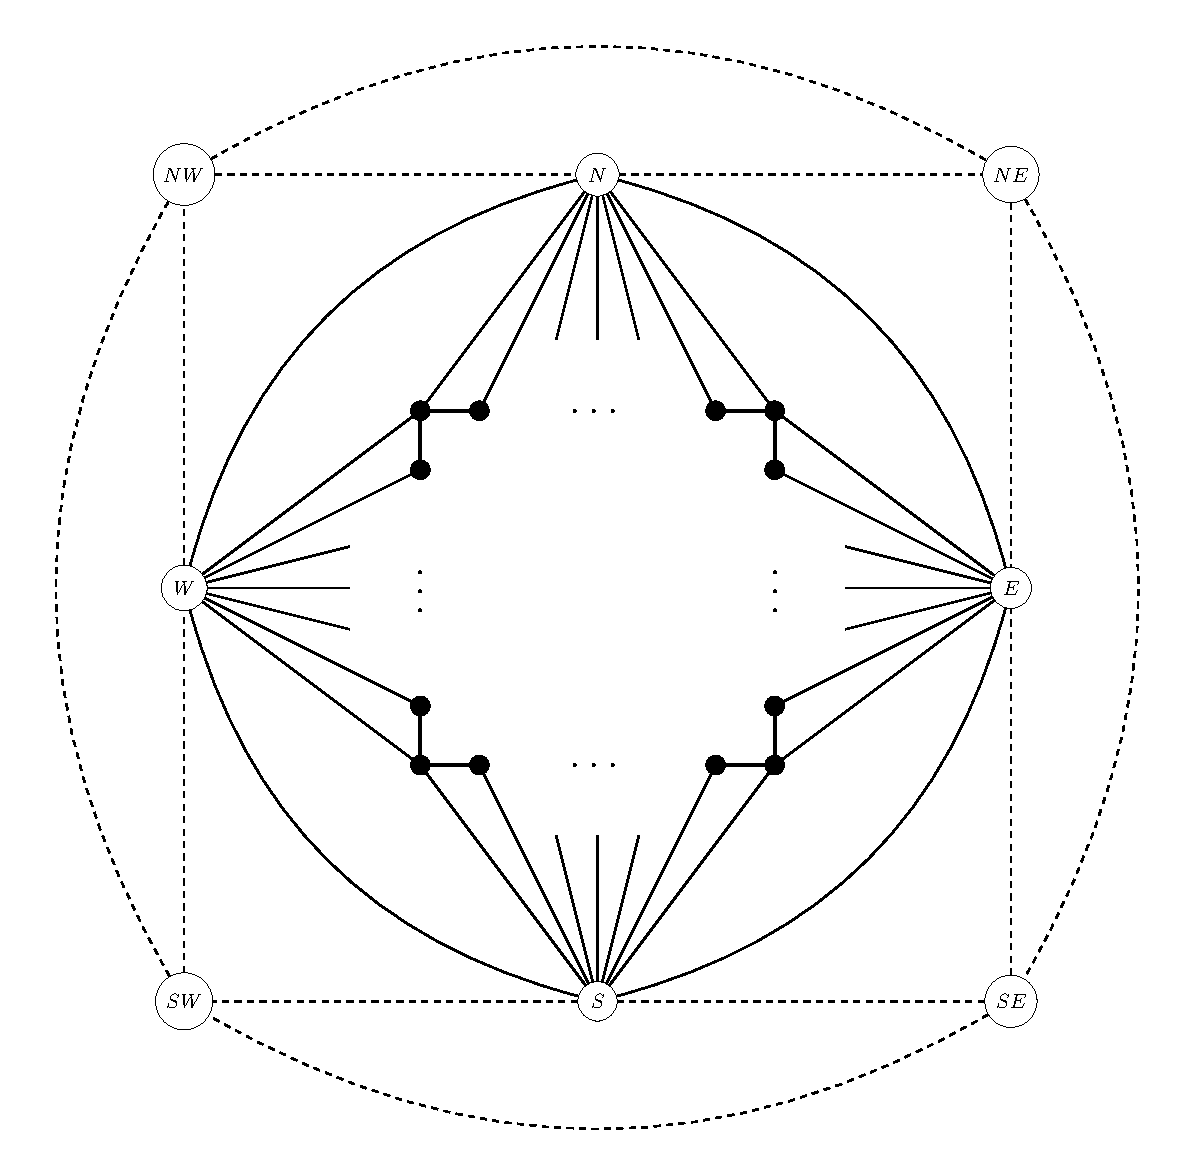
\includegraphics[scale=0.5]{fixExtension/img/scafold}

  \caption{The construction of a scaffold. $G$ is displayed in thick lines and with closed vertices. An arbitrary extension $\ext G =H$ is then drawn with thin lines and open vertices. An extension of $H$ is then drawn with dashed edges and open vertices.
      \label{fig:scafold}}
  \end{figure}

  \begin{proof}[Proof of Theorem \ref{th:fixExtension}]
    The graph $H$ can have more then one extension but they all contain the separating $4$-cycle $\C= NESW$ thus by Lemma \ref{lm:fix:fourCycleInteriorColor} we see that, without loss of generality, the interior edges of $\C$ incident to $N$ and $S$ are colored red and those incident to $E$ or $W$ are colored blue. This is exactly as if we forced the extension $\ext G$
    \end{proof}

\subsection{An application: There are graphs that are $(2, \infty)$-sided}

  We will show this by providing an example graph $G$ with a fixed extension $\ext G$ which we can do according to Theorem \ref{th:fixExtension}. Consider the graph in Figure \ref{fig:2manysidedLowerBound}. Note that most of the interior vertices are of degree $4$ and thus the largest part of any regular edge labeling is forced. Those edges that are forced to have a certain color are already colored in Figure \ref{fig:2manysidedLowerBound}.


  \begin{figure}[h!]
  \centering
  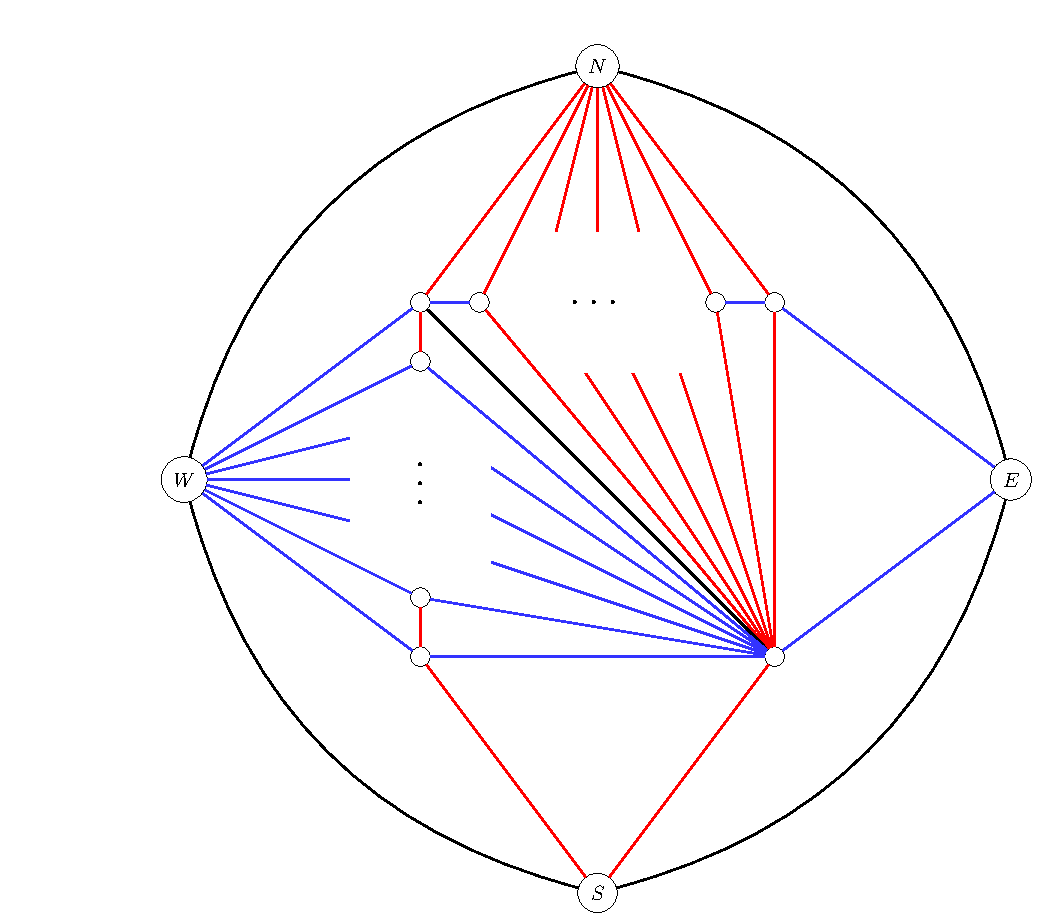
\includegraphics[scale=.5]{fixExtension/img/2manysidedLowerBound}

  \caption{The fixed extension $\ext G$
      \label{fig:2manysidedLowerBound}}
  \end{figure}

  The only edge for which we have freedom to choose a color is the diagonal edge of $G$. However, if we color this edge blue we get a red $(2, \infty)$ cycle and if we color this edge red we get a blue $(2, \infty)$ cycle. In both cases we will thus obtain a $(2,\infty)$-sided segment in our dual.

\subsection{Another application: There are graphs that are $(\infty, \infty)$-sided}
  \label{ss:fix:manymany}
  We will later see that all these graphs have adjacent maximal $4$-cycles.

  We consider the graph $G$ with extension $\ext G$ given in Figure \ref{fig:fix:manymany0}. Note that this graph has two adjacent maximal separating $4$-cycles. These are both marked by thick lines in Figure \ref{fig:fix:manymany0}.

  \begin{figure}[h]
    \centering
    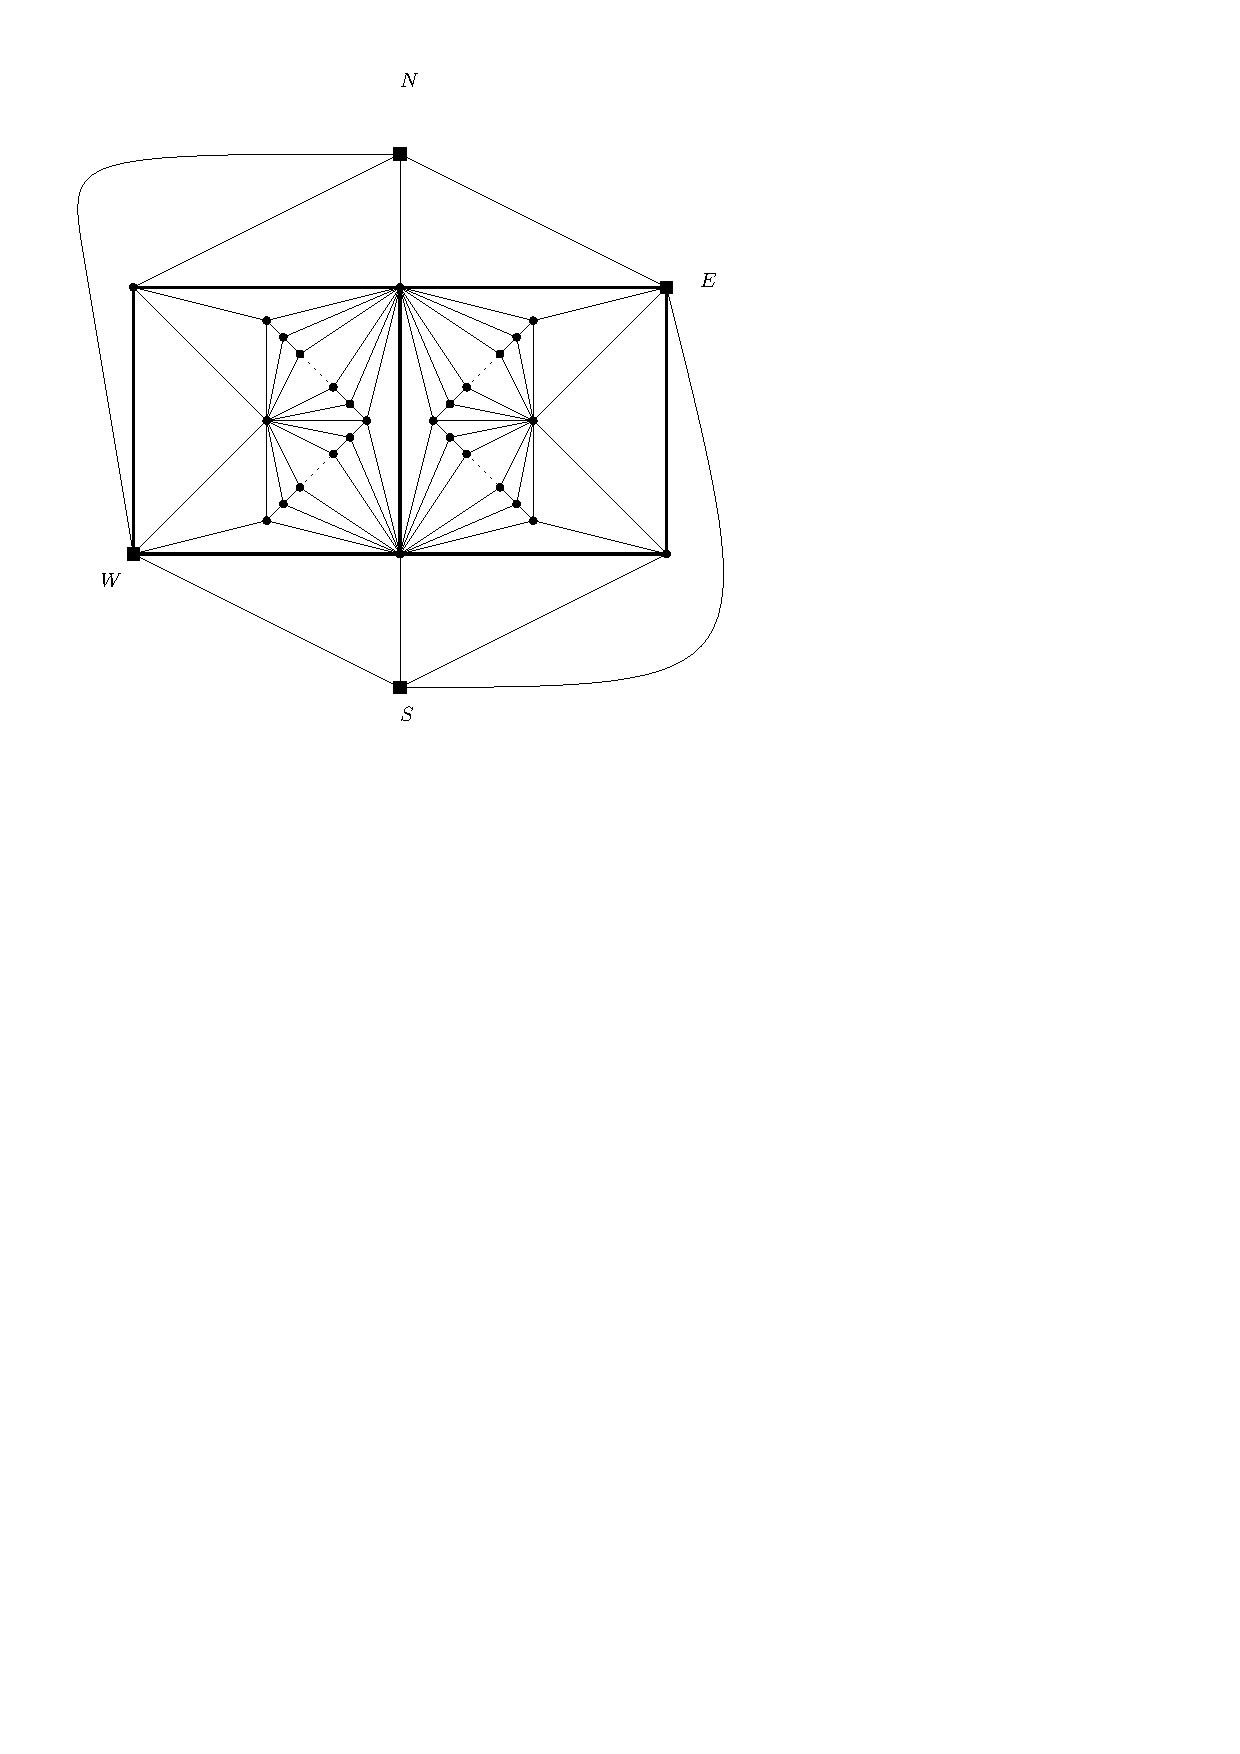
\includegraphics[scale=1]{fixExtension/img/manymanybase}
    \caption{}
    \label{fig:fix:manymany0}
  \end{figure}

  This graph has a lot of forced coloring. These forced colorings are performed in Figure \ref{fig:fix:coloring}. First we color the edges incident with the poles in accordance with the exterior vertex condition. Subsequently we propagate the coloring along both maximal separating $4$-cyles in accordance whit Lemma \ref{lm:fix:fourCycleInteriorColor} and finally we color the edges in triangles that have the other two edges colored in the same color. We can do this due to the fact that traingles in a regualar edge lableing are not mono-colored by Lemma \ref{lm:rel:noMonoColoredTriangles}.


  \begin{figure}[h]
    \centering

    \begin{subfigure}[t]{0.3\textwidth}
      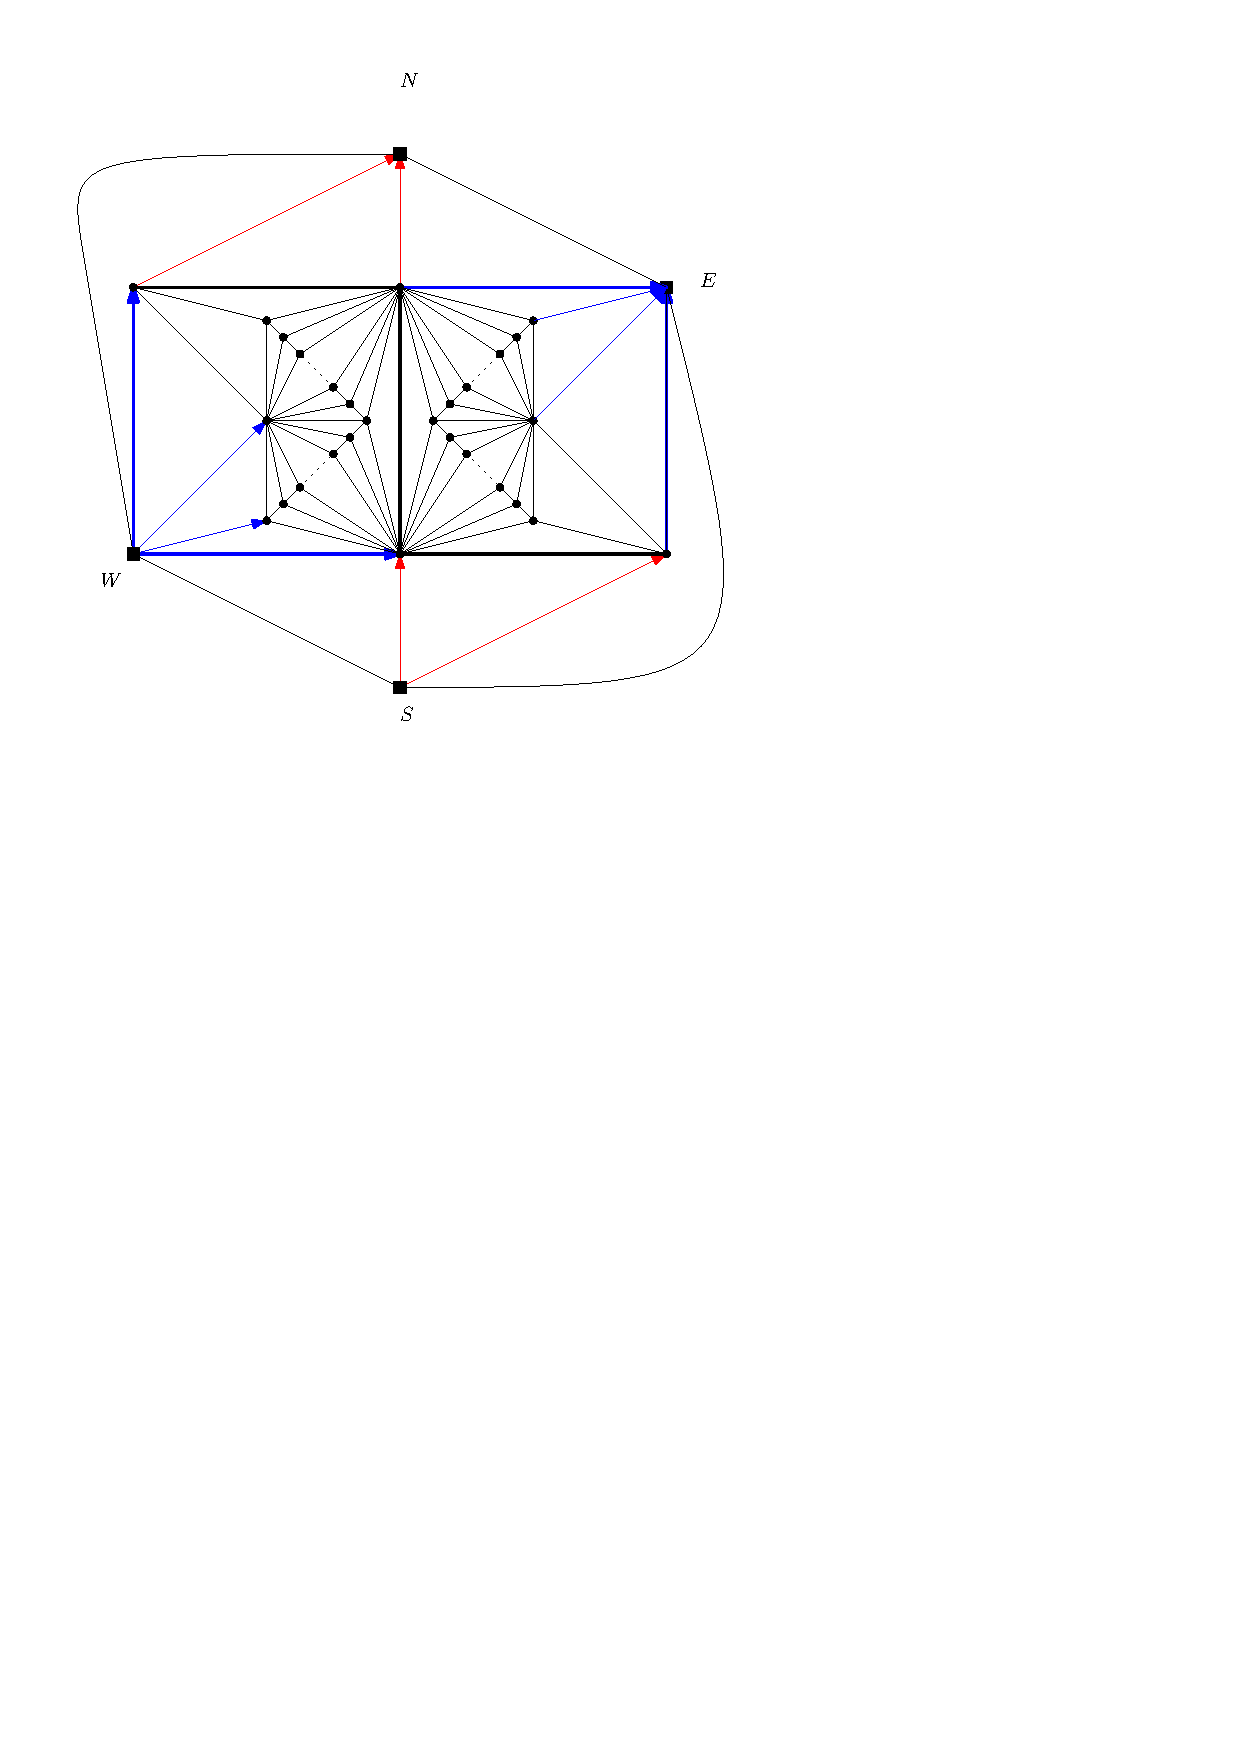
\includegraphics[width=\textwidth]{fixExtension/img/manymany1}
      \caption{Coloring the edges adjacent to the poles}
      \label{fig:fix:manymany1}
    \end{subfigure}
    \quad
    \begin{subfigure}[t]{0.3\textwidth}
      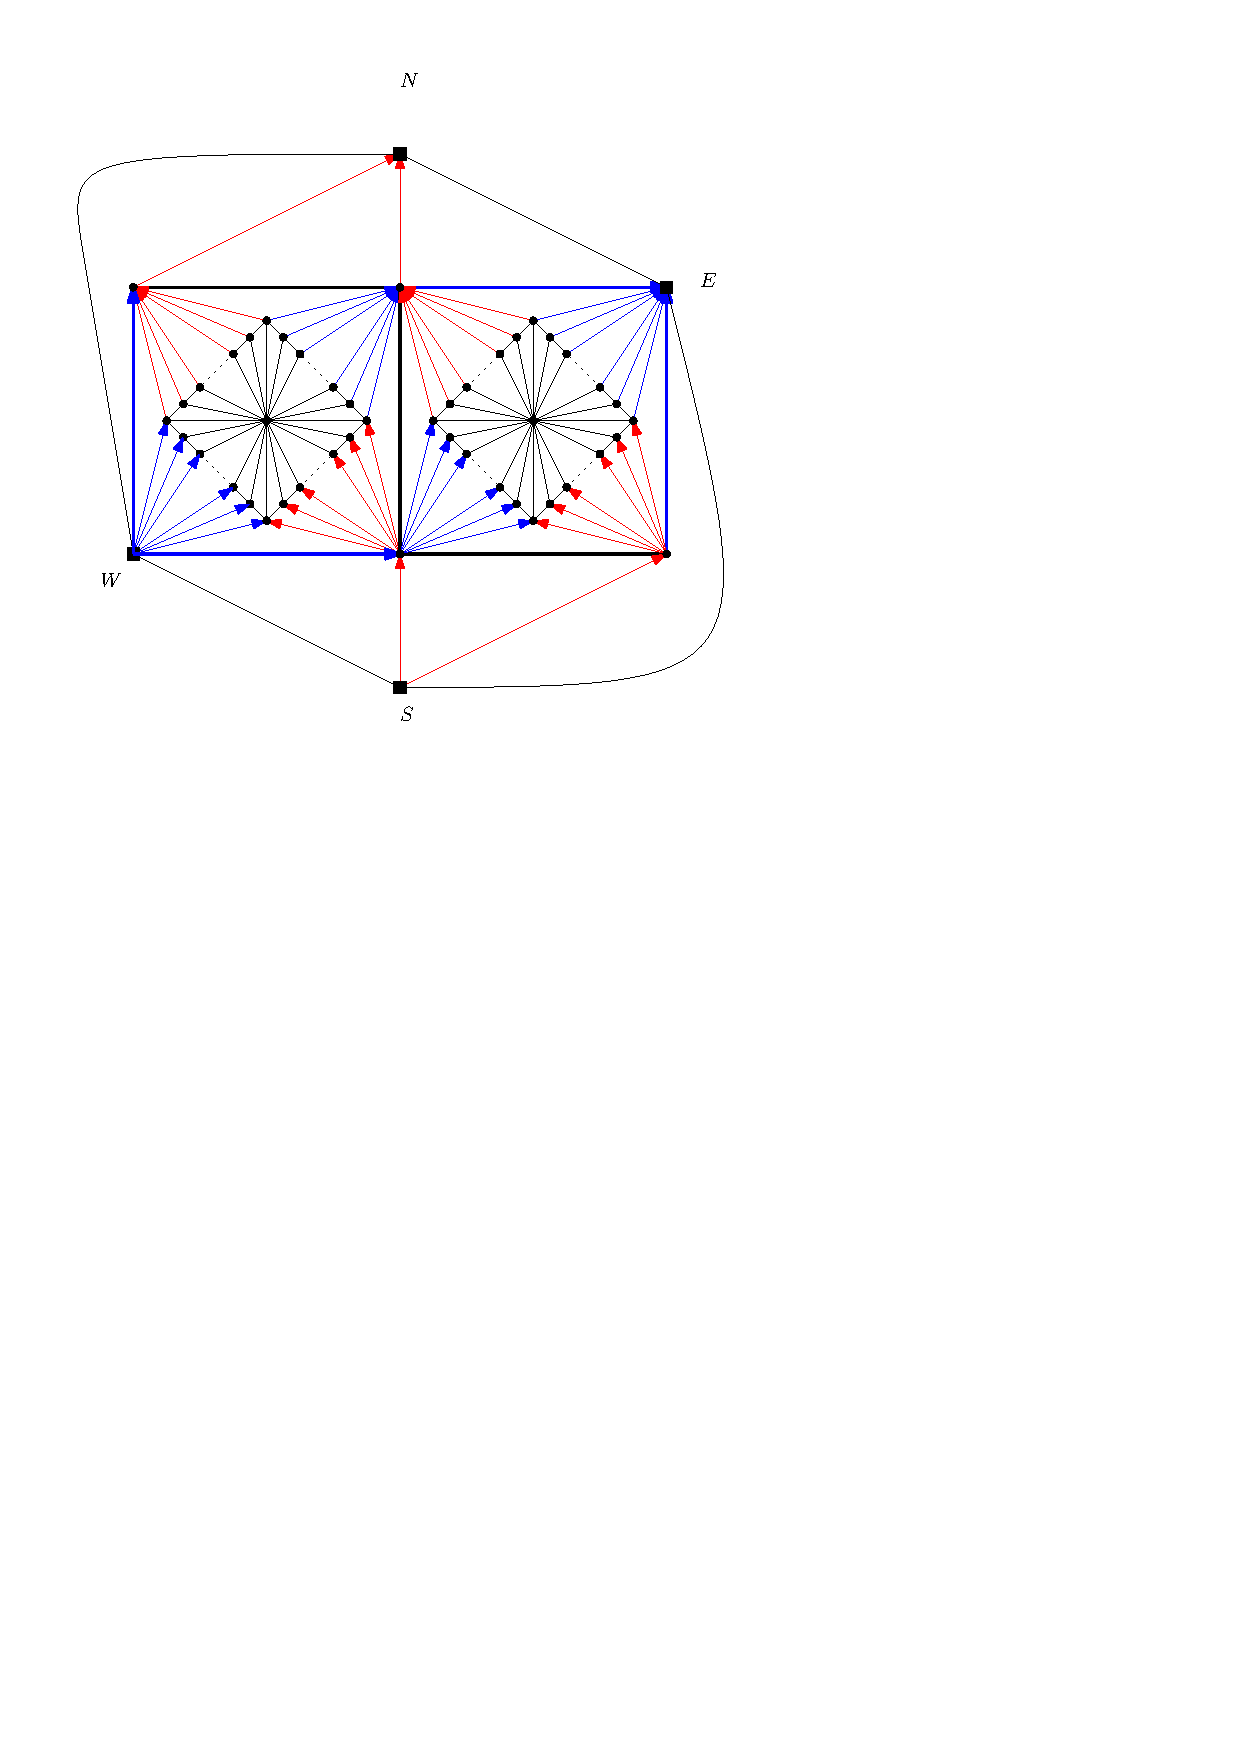
\includegraphics[width=\textwidth]{fixExtension/img/manymany2}
      \caption{Propagate trough the $4$-cycle}
      \label{fig:fix:manymany2}
    \end{subfigure}
    \quad
    \begin{subfigure}[t]{0.3\textwidth}
      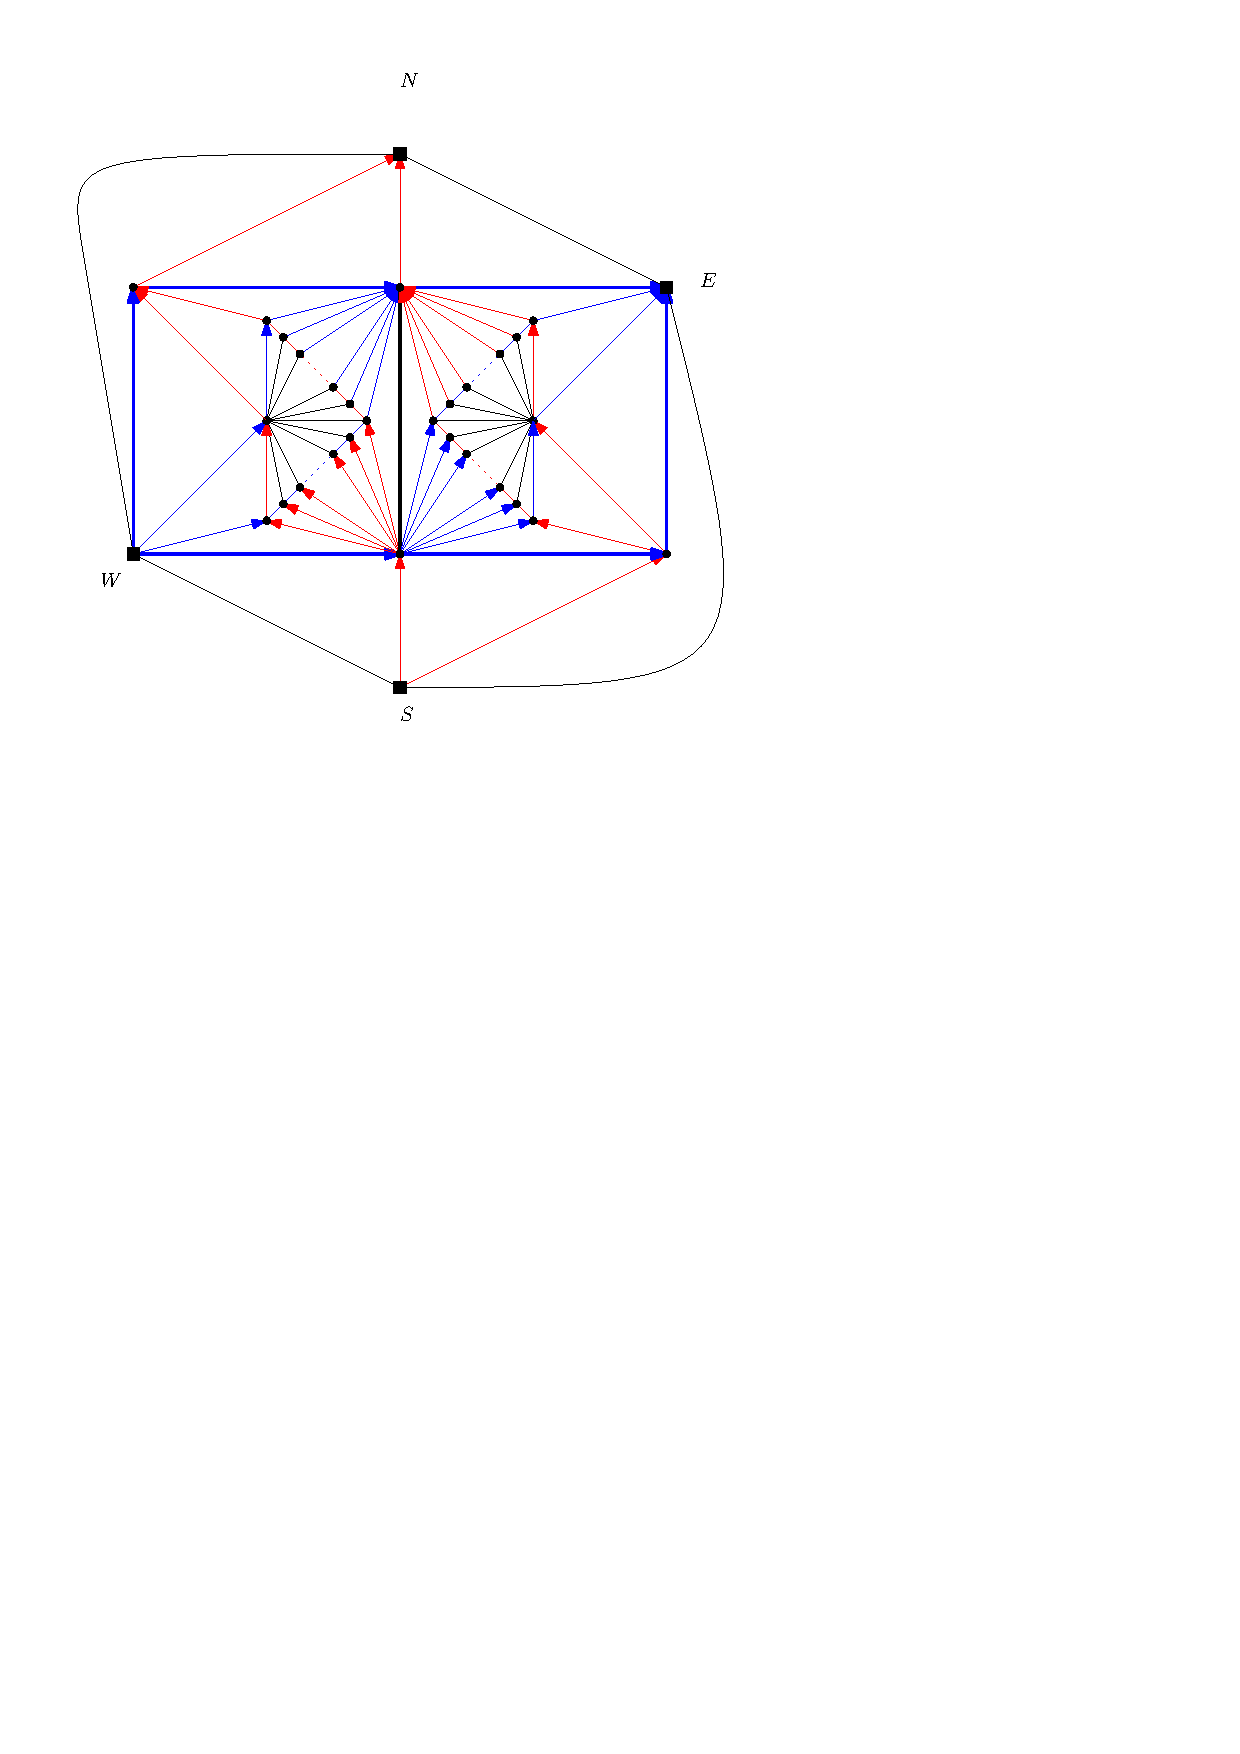
\includegraphics[width=\textwidth]{fixExtension/img/manymany3}
      \caption{Color such that there are no mono-colored triangles}
      \label{fig:fix:manymany3}
    \end{subfigure}
    \caption{Coloring the graph}
    \label{fig:fix:coloring}
  \end{figure}

   \fxwarning{TODO Show what is wrong with coloring}



  \begin{figure}[h]
    \centering
    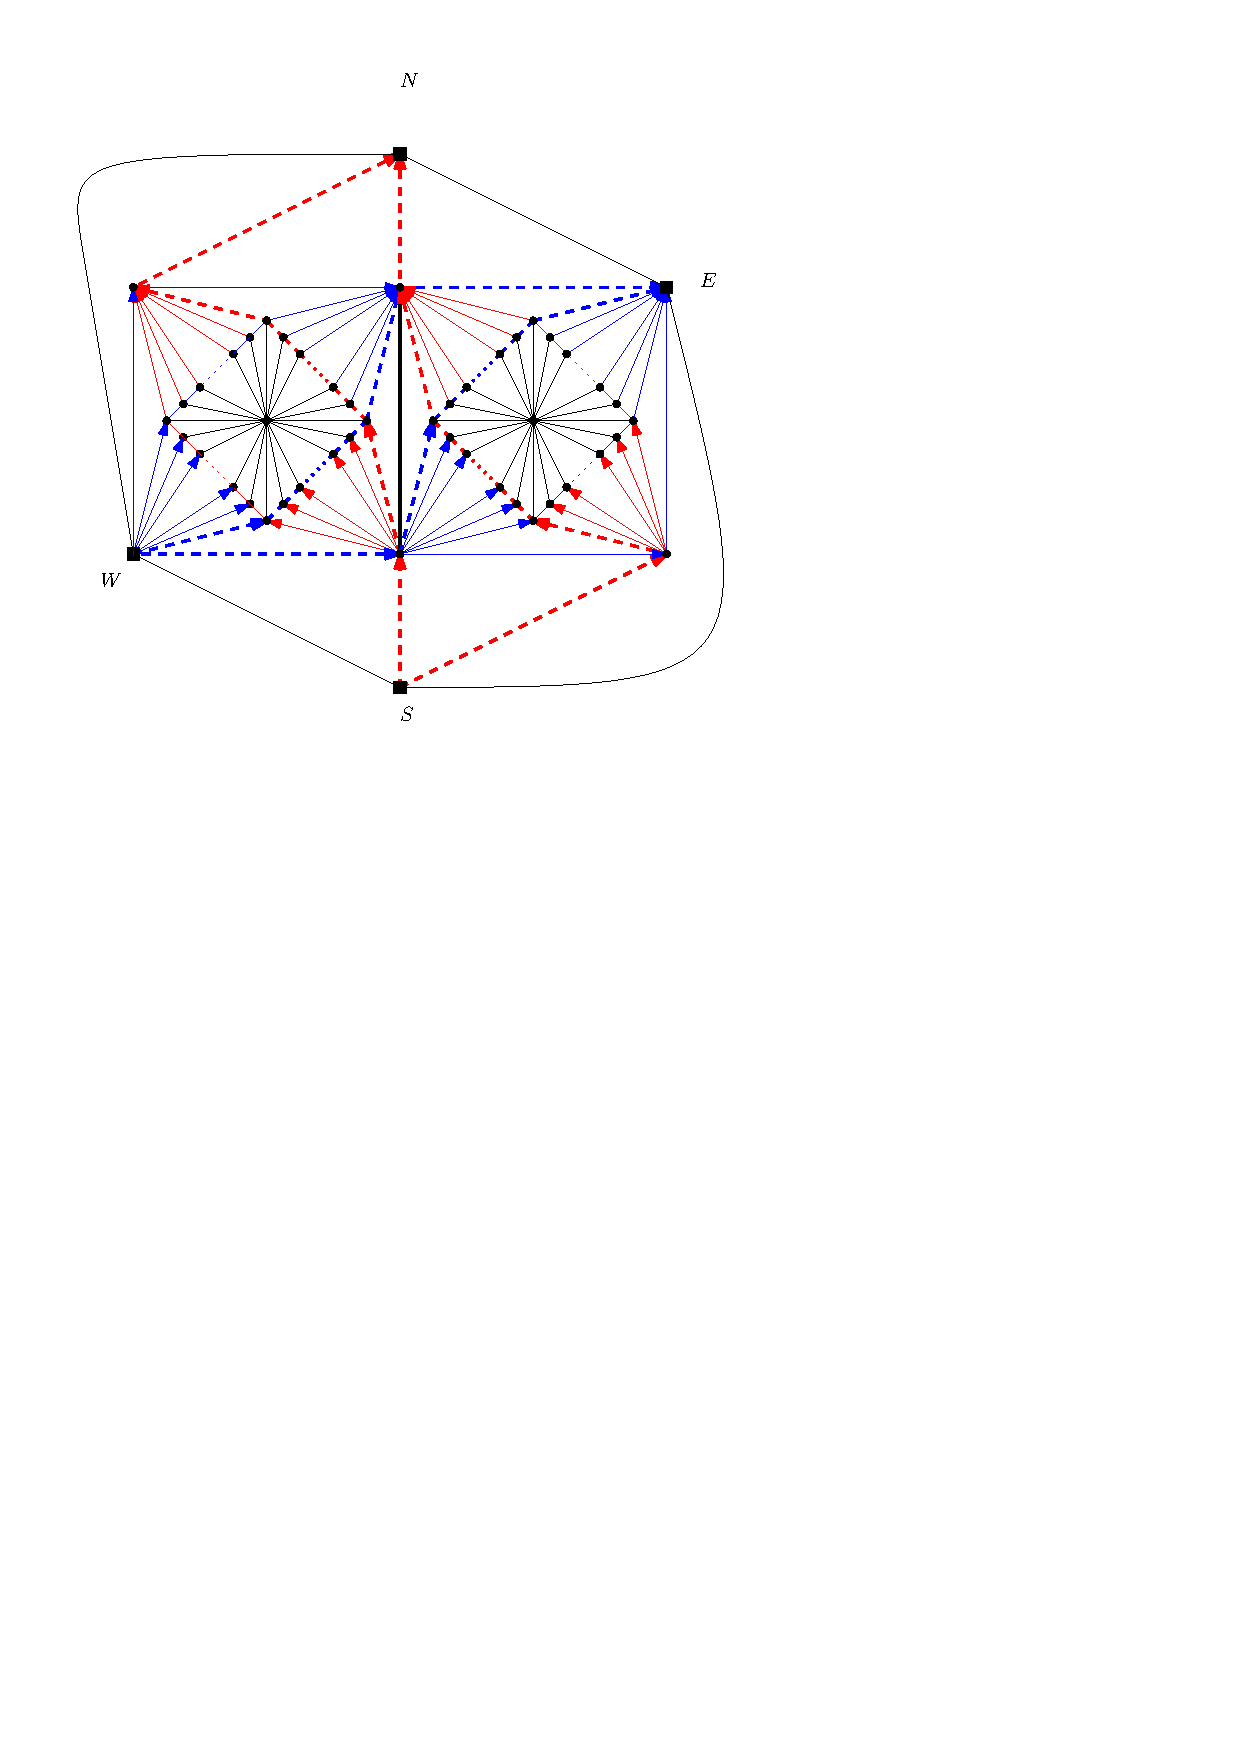
\includegraphics[scale=1]{fixExtension/img/manymany4}
    \caption{}
    \label{fig:fix:manymany4}
  \end{figure}
